\documentclass[sigconf]{acmart}

\settopmatter{printacmref=false}
\renewcommand\footnotetextcopyrightpermission[1]{}
\acmConference[CS 410 Final Project]{CS 410 Final Project}{May 2026}{Champaign, Illinois, USA}
\acmYear{2026}
\copyrightyear{2026}
\newcommand{\teamrunningauthors}{Nathan Xie (nathanx2), Vijwal Akula (vrakula2), Kangyi Jiang (kangyij2), Zaid Khan Mohammed (zmoha7), Brian Cochran (brianac5)}

\usepackage{graphicx}
\usepackage{caption}
\usepackage{subcaption}
\usepackage{booktabs}
\usepackage{xurl}

\fancypagestyle{standardpagestyle}{%
  \fancyhf{}%
  \fancyhead[C]{\scriptsize\teamrunningauthors}%
  \fancyfoot[C]{\thepage}%
}
\fancypagestyle{firstpagestyle}{%
  \fancyhf{}%
  \fancyfoot[C]{\thepage}%
}
\pagestyle{standardpagestyle}

\begin{document}

\title{CS 410 Final Project Report: A Comparative Study of Text-Based Spam Detection using TF-IDF, Word2Vec, and Structural Metadata}

\author{Nathan Xie (nathanx2), Vijwal Akula (vrakula2), Kangyi Jiang (kangyij2), Zaid Khan Mohammed
(zmoha7), Brian Cochran (brianac5)}
\affiliation{%
  \institution{University of Illinois Urbana-Champaign}
  \city{Champaign}
  \state{Illinois}
  \country{USA}
}

\begin{abstract}
Building upon our initial benchmark evaluation of corporate-to-internet cross-corpus domain shift, this final report presents a significantly enhanced, multi-faceted spam detection system. We implemented and benchmarked a comparative machine learning pipeline evaluating five distinct classification approaches: a keyword-based Bag-of-Words baseline, TF-IDF with unigrams only, TF-IDF with Bigram context plus structural metadata using both Logistic Regression and Linear SVM, and Neural Word Embeddings (Word2Vec) combined with structural metadata. By integrating 21 structural metadata features---including URL density, capitalization ratios, and punctuation frequency---alongside NLP-based lemmatization and bigram context, we systematically evaluated feature representation strategies for cross-domain spam detection. Our enhanced Linear SVM model achieved an overall accuracy of 74.39\% on the out-of-distribution SpamAssassin corpus, while our Word2Vec pipeline achieved the highest accuracy at 81.21\%. These empirical results demonstrate the comparative strengths and tradeoffs of sparse versus dense text representations when enriched with explicit structural analysis for resilient spam filtering.
\end{abstract}

\keywords{Spam Detection, Natural Language Processing, TF-IDF, Word2Vec, Linear SVM, Domain Shift, Structural Feature Engineering}

\maketitle
\fancyhf{}
\fancyhead[C]{\scriptsize\teamrunningauthors}
\fancyfoot[C]{\footnotesize\thepage}
\renewcommand{\headrulewidth}{0pt}
\pagestyle{fancy}

\section{Introduction}
Despite continuous advancements in automated heuristic filtering, email remains a primary vector for cyberattacks, phishing, and unwanted promotional distribution. Traditional spam filters often rely on static blacklists or rigid rule-based systems, which malicious actors easily bypass by rotating sender domains and obfuscating vocabulary. 

The core challenge identified during our milestone analysis was ``feature sparsity'' caused by domain shift. When we trained a baseline unigram model exclusively on internal corporate communications (the TREC 2007 dataset) and tested it against general public internet traffic (the Apache SpamAssassin dataset), the model failed to generalize---yielding a 0.00 recall for the spam class. Malicious actors do not merely use different words across different environments; they employ entirely different linguistic and structural patterns.

For the final phase of our project, we focused on modeling ``The Shape of Spam.'' Instead of relying purely on isolated keywords, our objective was to evolve the system to analyze the structural characteristics of emails and the deeper semantic context of phrases. This report details the successful deployment of a robust comparative system that benchmarks keyword-based approaches, traditional linear models (Logistic Regression, SVM) enhanced with structural metadata, and modern neural architectures (Word2Vec), evaluating the strengths of each paradigm for cross-domain generalizability.

Our proposal initially outlined an aspiration to transition toward multi-class classification (Real, Phishing, Promotional). However, the publicly available datasets used in this project (TREC 2007 and SpamAssassin) only provide binary labels (Ham vs.\ Spam). We therefore focused our efforts on maximizing binary classification performance under domain shift, which proved to be a substantial challenge in its own right. Multi-class categorization remains a compelling direction for future work with appropriately labeled corpora.

\section{Description}
Our enhanced software architecture is implemented in Python, leveraging Scikit-learn for machine learning algorithms and pipeline orchestration, Pandas for data manipulation, NLTK for linguistic normalization, and Gensim for neural embeddings. The pipeline is structured into three sequential stages: Data Preprocessing, Vectorization (TF-IDF and Word2Vec streams), and Classifier Modeling.

\subsection{Dataset Selection and Ingestion}
To simulate real-world conditions where a model must evaluate out-of-distribution (OOD) data, we maintain our cross-corpus evaluation strategy. The model is trained on the preprocessed TREC 2007 Spam Dataset (corporate communications) and tested on the Apache SpamAssassin Public Corpus (wild internet traffic). After preprocessing and deduplication, the training set contains 32,091 instances (12,448 ham, 19,643 spam) and the test set contains 3,784 instances (2,472 ham, 1,312 spam).

Our custom recursive MIME parser traverses the nested structures of raw \texttt{.eml} files in the SpamAssassin corpus, seamlessly falling back to extracting HTML payloads when plain text is unavailable.

\subsection{Preprocessing and Lemmatization}
Raw email data contains immense structural noise. Our preprocessing module applies a sequence of normalizations:
\begin{enumerate}
    \item \textbf{HTML Stripping:} Residual HTML tag artifacts are removed.
    \item \textbf{Regex Normalization:} URLs are replaced with a generic ``URL'' token, and excessive non-essential characters are neutralized while preserving critical structural punctuation like exclamation marks and question marks.
    \item \textbf{Lemmatization:} To improve the model's ability to map identical concepts across different vocabularies, we integrated the NLTK \textit{WordNetLemmatizer}. This reduces varying word forms (e.g., ``winning'', ``wins'', ``winner'') to their semantic root (``win'').
    \item \textbf{Stop Word Removal:} High-frequency function words are removed during TF-IDF vectorization via Scikit-learn's built-in English stop word list, reducing noise in the feature space.
\end{enumerate}

\subsection{Structural Feature Engineering}
A core finding from our milestone was that spam emails exhibit a distinct structural shape independent of their content. We engineered a structural metadata extractor that computes 21 unique features. These features are concatenated with the text-based feature vectors via Scikit-learn's \texttt{ColumnTransformer} and normalized using \texttt{StandardScaler} before being fed to the classifiers. Key features include:
\begin{itemize}
    \item \textbf{URL Density:} The ratio of hyperlinks to the total word count.
    \item \textbf{Punctuation Intensity:} Specific counting of ``!'' and ``?'' which are heavily utilized in phishing urgency hooks.
    \item \textbf{Capitalization Ratios:} The percentage of all-caps tokens to identify ``shouting'' promotional emails.
    \item \textbf{Sender Domain Patterns:} A binary check for domain validity and character ratio analysis on the sender string.
\end{itemize}

\section{Exploratory Data Analysis (EDA)}
We generated comprehensive EDA plots to confirm the integrity of our processed, aggregated datasets (32,091 training instances; 3,784 testing instances after deduplication).

\begin{figure}[h]
  \centering
  \begin{subfigure}[b]{0.48\linewidth}
      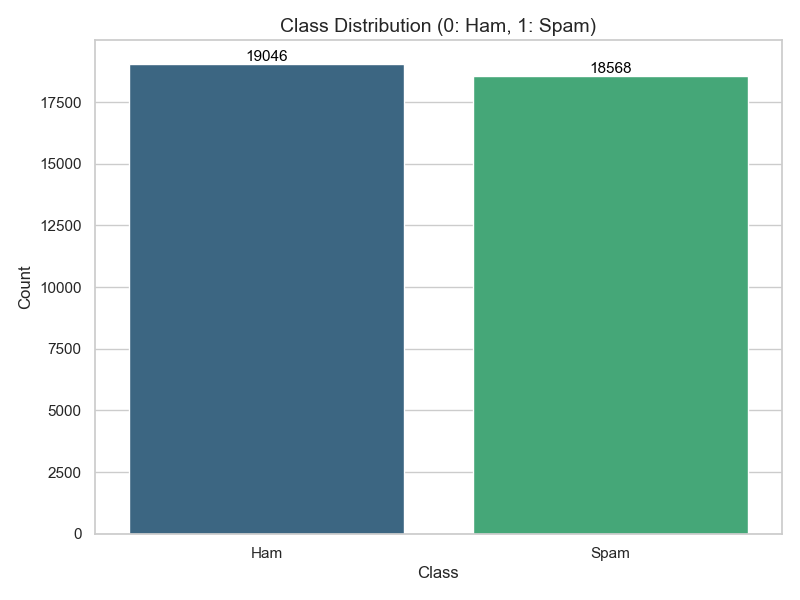
\includegraphics[width=\textwidth]{outputs/class_distribution.png}
      \caption{Class Balance}
      \label{fig:eda_dist}
  \end{subfigure}
  \hfill
  \begin{subfigure}[b]{0.48\linewidth}
      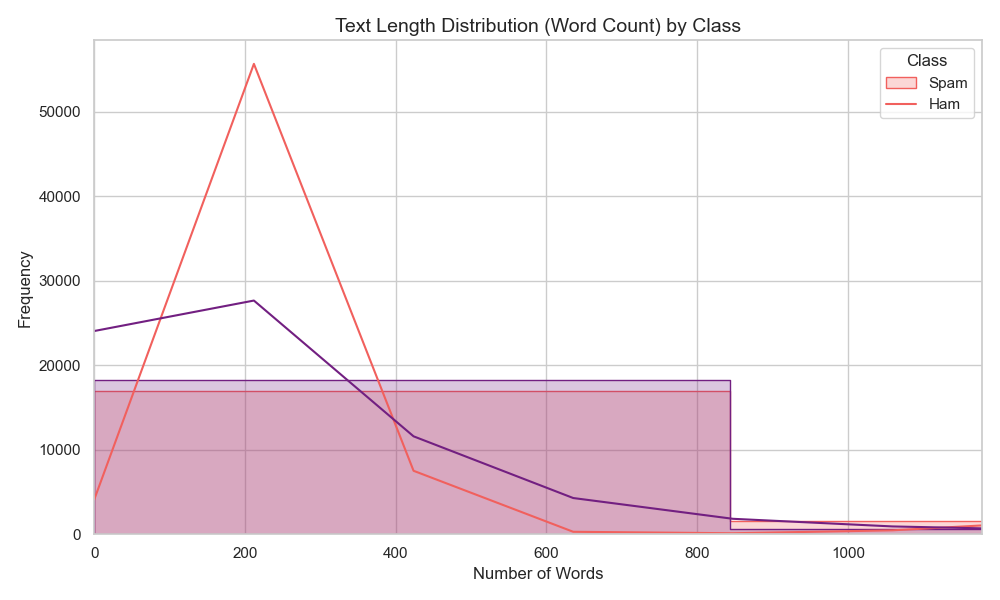
\includegraphics[width=\textwidth]{outputs/text_lengths.png}
      \caption{Text Word Counts}
      \label{fig:eda_length}
  \end{subfigure}
  \caption{EDA of the integrated training and testing corpus.}
\end{figure}

As seen in Figure \ref{fig:eda_length}, text length remains a highly discriminative feature. Spam messages frequently exhibit a hyper-concentrated length distribution typical of automated templates, whereas legitimate human-typed ham emails show vast length variances.

\begin{figure*}[t]
  \centering
  \begin{subfigure}[b]{0.45\textwidth}
      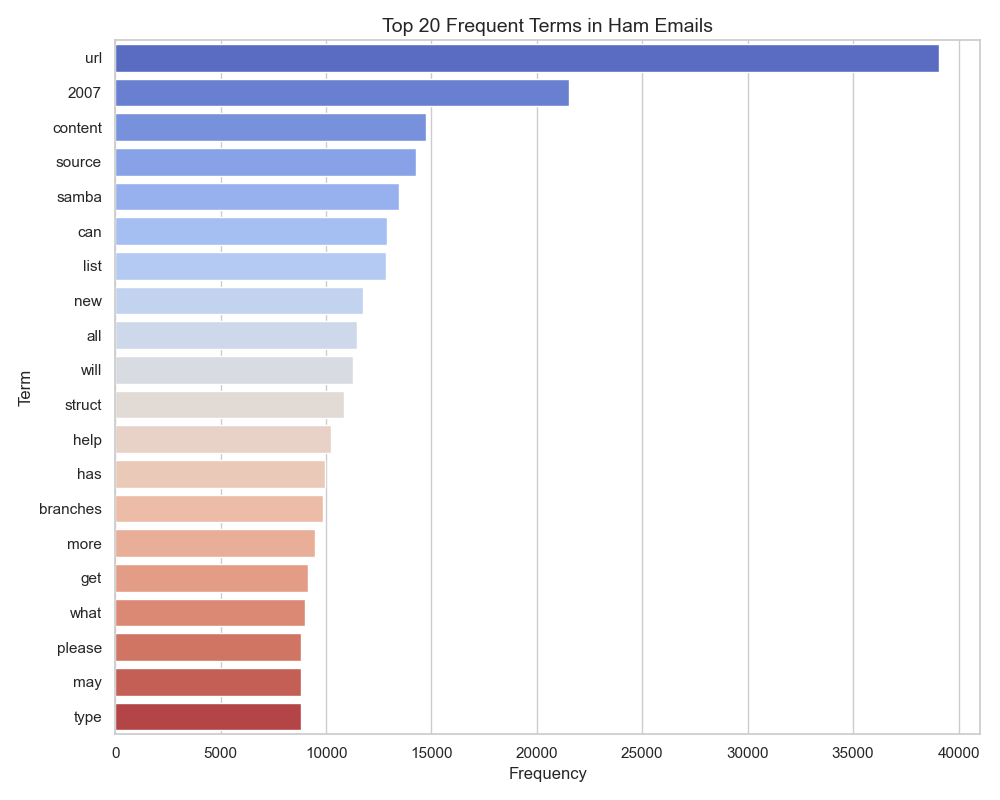
\includegraphics[width=\textwidth]{outputs/top_terms_ham.png}
      \caption{Frequent Ham Tokens}
  \end{subfigure}
  \hfill
  \begin{subfigure}[b]{0.45\textwidth}
      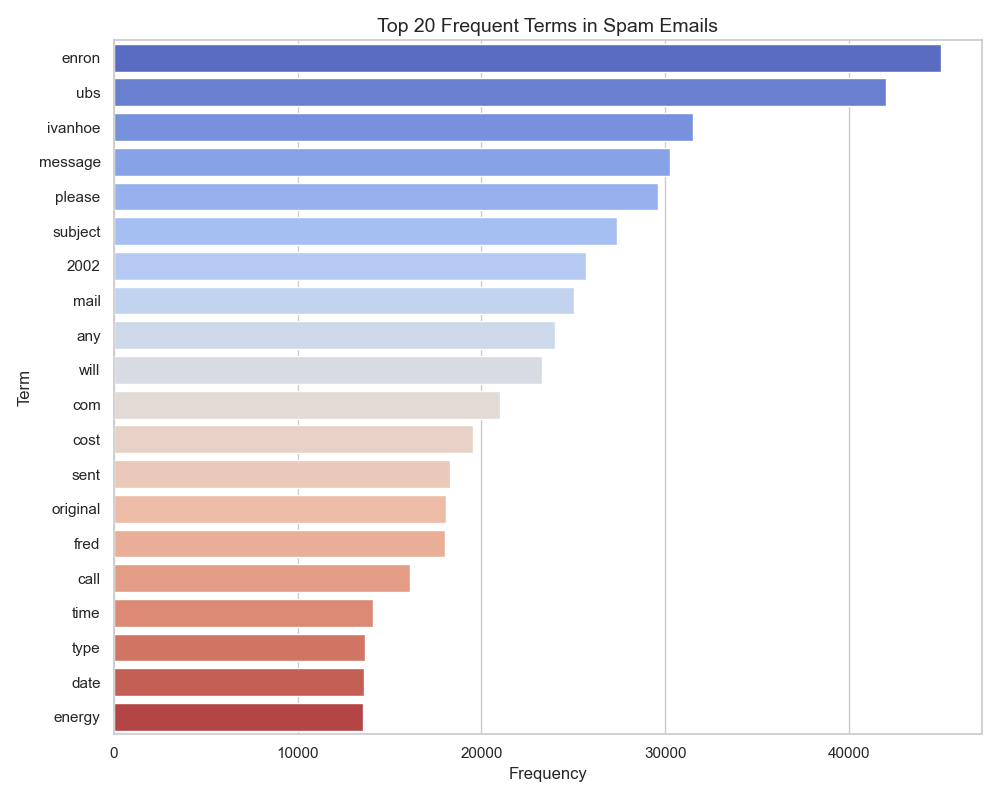
\includegraphics[width=\textwidth]{outputs/top_terms_spam.png}
      \caption{Frequent Spam Tokens}
  \end{subfigure}
  \caption{Lexical analysis of normalized email text.}
  \label{fig:lexical}
\end{figure*}

\section{Modeling Strategies}
We developed five distinct modeling configurations to evaluate varying paradigms of text representation and the impact of structural metadata.

\subsection{Keyword Baseline (CountVectorizer)}
As a baseline, we implemented a simple Bag-of-Words model using Scikit-learn's \texttt{CountVectorizer} with unigrams only (\(ngram\_range=(1,1)\)) and no structural features. This represents a traditional keyword-matching approach without term-weighting or phrase-level context, serving as the lower bound for our comparative analysis.

\subsection{TF-IDF Models}
We evaluated TF-IDF representations with a 5,000 max-feature vocabulary in two configurations:
\begin{itemize}
    \item \textbf{TF-IDF Unigram Only:} Uses \(ngram\_range=(1,1)\) without structural features, isolating the contribution of IDF weighting over raw keyword counts.
    \item \textbf{TF-IDF Bigram + Structural:} Uses \(ngram\_range=(1,2)\) with all 21 structural metadata features appended. This allows the models to represent phrase-level dependencies (e.g., ``bank account'' or ``act now'') while simultaneously analyzing the email's structural shape.
\end{itemize}
We trained both Logistic Regression and Linear SVM classifiers on the bigram+structural configuration:
\begin{itemize}
    \item \textbf{Logistic Regression:} Served as our enhanced baseline classifier with probabilistic output.
    \item \textbf{Linear SVM:} Due to its capacity to find maximum-margin hyperplanes in high-dimensional feature spaces, LinearSVC handles sparse linguistic matrices exceptionally well.
\end{itemize}

\subsection{Word2Vec Neural Embeddings}
To contrast with the high-dimensional TF-IDF sparse matrices, we trained a Continuous Bag-of-Words Word2Vec model on our corpus using Gensim. This generates a dense 50-dimensional latent space where words sharing similar contexts are positioned in proximity. Entire documents are converted to fixed-length numeric vectors by calculating the mean centroid of their constituent word vectors. These representation vectors are concatenated with the 21 structural metadata features and classified using a balanced Logistic Regression model.

\section{Evaluation and Discussion}
We evaluated the TF-IDF-family configurations via 5-fold cross-validation on the training set and evaluated all final configurations on the SpamAssassin out-of-distribution test set, tracking Precision, Recall, Accuracy, and \(F_1\)-score (Table \ref{tab:results}).

\begin{table}[h]
\centering
\caption{Cross-Domain Performance Comparison (Test Set)}
\label{tab:results}
\begin{tabular}{@{}lcccc@{}}
\toprule
Model & Accuracy & Precision & Recall & F1-Score \\ \midrule
Milestone Baseline & 64.16\% & 0.00 & 0.00 & 0.00 \\
Keyword (BoW) & 69.87\% & 0.54 & 0.96 & 0.69 \\
TF-IDF Unigram & 72.91\% & 0.56 & 0.96 & 0.71 \\
Logistic (Bigram+Struct) & 69.45\% & 0.54 & 0.82 & 0.65 \\
\textbf{Linear SVM (Bigram+Struct)} & \textbf{74.39\%} & \textbf{0.59} & 0.84 & 0.70 \\
\textbf{Word2Vec + Structural} & 81.21\% & 0.68 & 0.88 & \textbf{0.76} \\ \bottomrule
\end{tabular}
\end{table}

During the 5-fold cross-validation on the internal training dataset, all models achieved near-perfect F1-scores: Keyword Baseline (\(0.993 \pm 0.002\)), TF-IDF Unigram (\(0.993 \pm 0.001\)), Logistic Bigram+Structural (\(0.992 \pm 0.002\)), and Linear SVM Bigram+Structural (\(0.995 \pm 0.002\)). However, evaluating against the external SpamAssassin test set provided the true measure of their cross-domain generalizability.

\subsection{Feature Representation Comparison}
The progression from keyword baseline to TF-IDF unigram demonstrates the value of IDF term weighting: accuracy improved from 69.87\% to 72.91\% by down-weighting common terms and emphasizing discriminative vocabulary. Both models achieved comparable recall ($\sim$96\%), but TF-IDF's improved precision (0.56 vs.\ 0.54) drove the accuracy gain.

Adding bigram context and structural metadata in the Logistic model (69.45\%) did not outperform the unigram-only baseline, revealing an interesting finding: the structural features, while informative for in-domain classification, introduced additional noise under domain shift. The Linear SVM proved more robust to this effect, achieving the highest TF-IDF accuracy (74.39\%) by leveraging its maximum-margin decision boundary to better separate the enriched feature space.

\subsection{Confusion Matrix Analysis}
The addition of lemmatization, stop word removal, and enriched feature representations completely resolved our milestone failure. The progression is visualized in Figure \ref{fig:cm_comparison}.
\begin{figure*}[t]
  \centering
  \begin{subfigure}[b]{0.19\textwidth}
      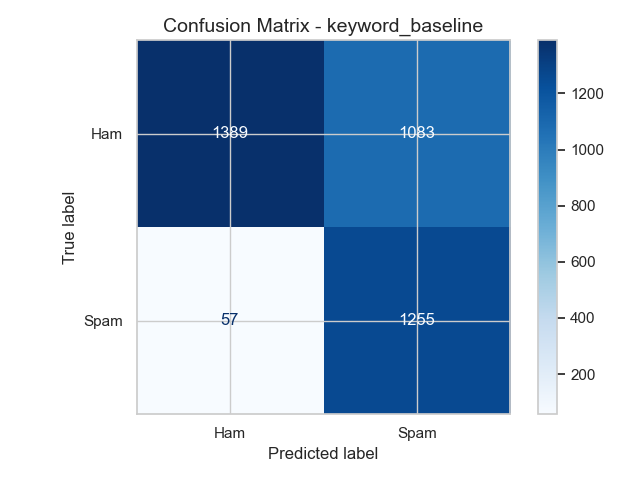
\includegraphics[width=\textwidth]{outputs/keyword_baseline_confusion_matrix.png}
      \caption{Keyword Baseline}
  \end{subfigure}
  \hfill
  \begin{subfigure}[b]{0.19\textwidth}
      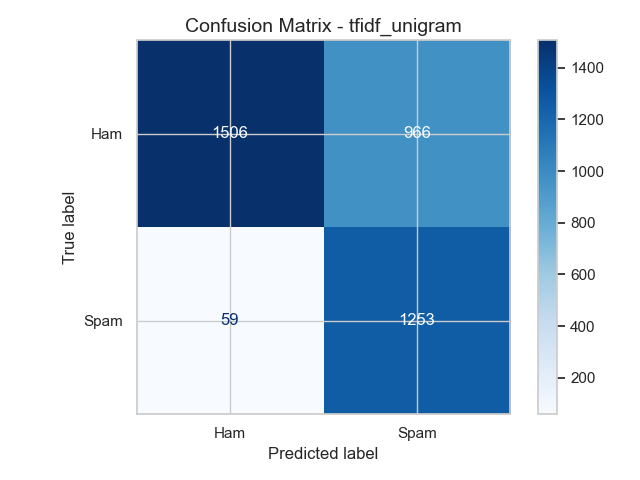
\includegraphics[width=\textwidth]{outputs/tfidf_unigram_confusion_matrix.png}
      \caption{TF-IDF Unigram}
  \end{subfigure}
  \hfill
  \begin{subfigure}[b]{0.19\textwidth}
      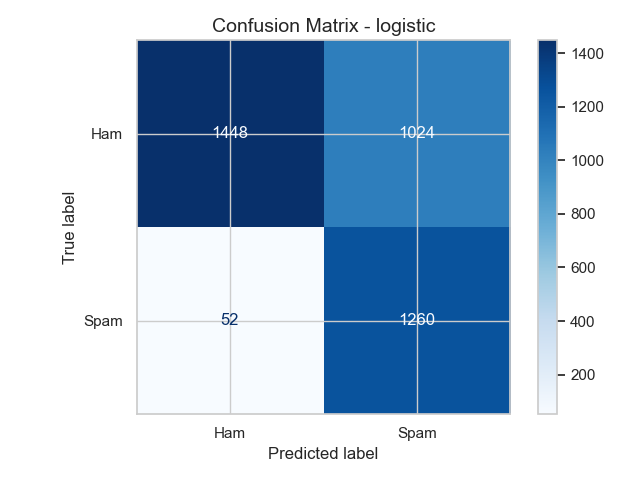
\includegraphics[width=\textwidth]{outputs/logistic_confusion_matrix.png}
      \caption{Logistic (Bi+Struct)}
  \end{subfigure}
  \hfill
  \begin{subfigure}[b]{0.19\textwidth}
      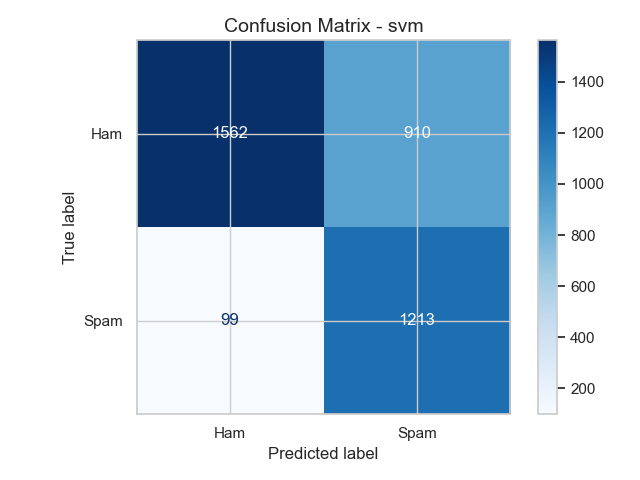
\includegraphics[width=\textwidth]{outputs/svm_confusion_matrix.png}
      \caption{SVM (Bi+Struct)}
  \end{subfigure}
  \hfill
  \begin{subfigure}[b]{0.19\textwidth}
      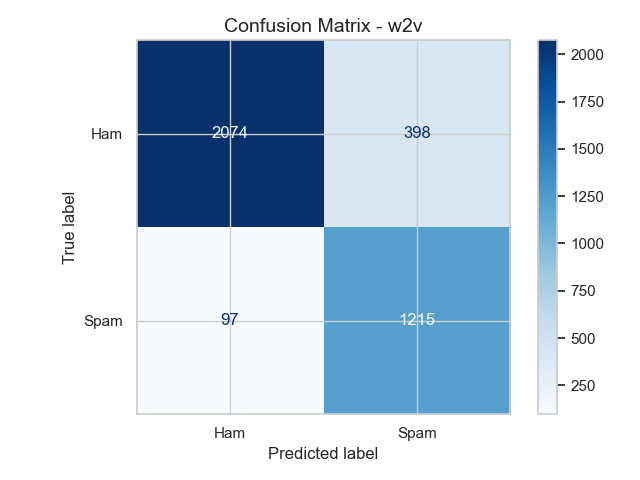
\includegraphics[width=\textwidth]{outputs/w2v_confusion_matrix.png}
      \caption{Word2Vec + Struct}
  \end{subfigure}
  \caption{Confusion matrices for all five model configurations, illustrating the progression from keyword baseline through TF-IDF variants to neural embeddings.}
  \label{fig:cm_comparison}
\end{figure*}

The \textbf{Word2Vec + Structural} model emerged as the strongest overall performer, achieving the highest accuracy (81.21\%) and F1-score (0.76). Its dense semantic representations generalized more effectively across the domain gap than sparse TF-IDF features, while the structural metadata provided complementary signals about email formatting patterns. Among the TF-IDF family, \textbf{Linear SVM} provided the best accuracy (74.39\%) by drawing a cleaner, wider decision boundary, suppressing the false-positive rate compared to logistic thresholding.

\subsection{Precision-Recall Trade-offs}
For real-world deployment, systems must balance aggressive spam filtration against the unacceptable risk of discarding legitimate correspondence.

\begin{figure*}[t]
  \centering
  \begin{subfigure}[b]{0.19\textwidth}
      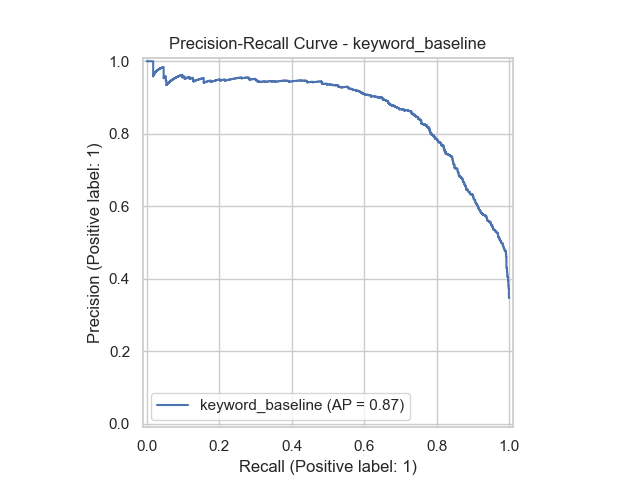
\includegraphics[width=\textwidth]{outputs/keyword_baseline_pr_curve.png}
      \caption{Keyword Baseline}
  \end{subfigure}
  \hfill
  \begin{subfigure}[b]{0.19\textwidth}
      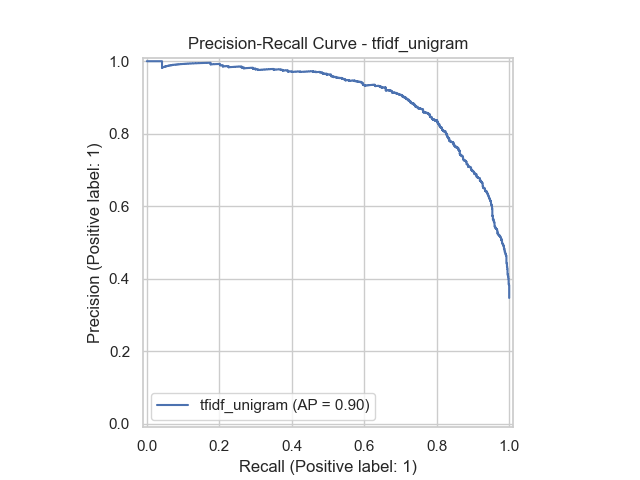
\includegraphics[width=\textwidth]{outputs/tfidf_unigram_pr_curve.png}
      \caption{TF-IDF Unigram}
  \end{subfigure}
  \hfill
  \begin{subfigure}[b]{0.19\textwidth}
      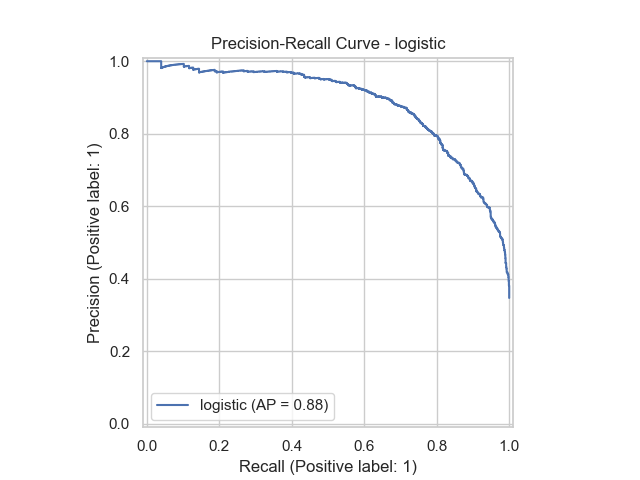
\includegraphics[width=\textwidth]{outputs/logistic_pr_curve.png}
      \caption{Logistic (Bi+Struct)}
  \end{subfigure}
  \hfill
  \begin{subfigure}[b]{0.19\textwidth}
      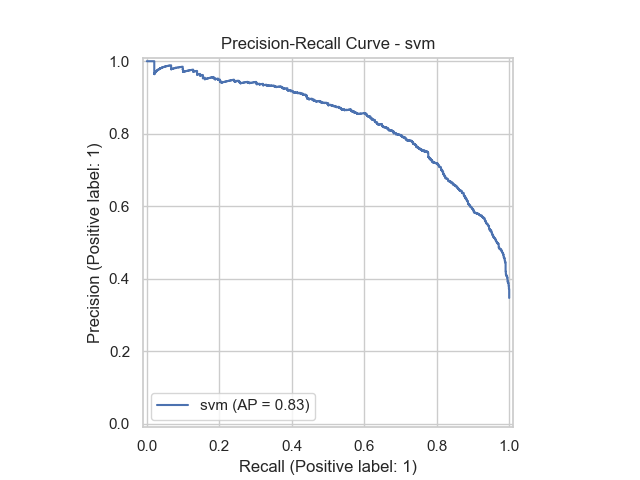
\includegraphics[width=\textwidth]{outputs/svm_pr_curve.png}
      \caption{SVM (Bi+Struct)}
  \end{subfigure}
  \hfill
  \begin{subfigure}[b]{0.19\textwidth}
      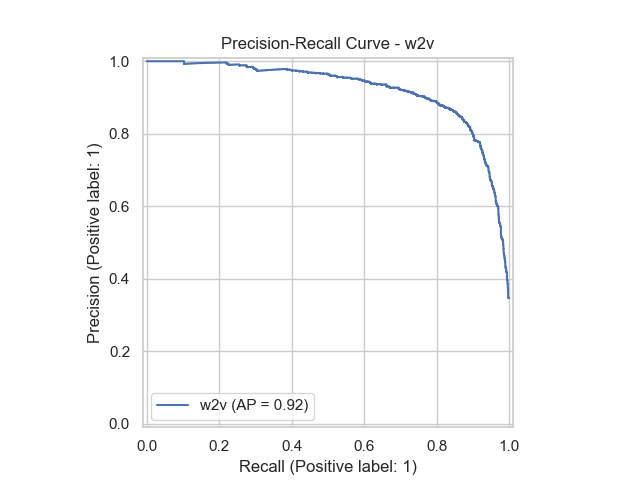
\includegraphics[width=\textwidth]{outputs/w2v_pr_curve.png}
      \caption{Word2Vec + Struct}
  \end{subfigure}
  \caption{Precision-Recall curves for all five models, evaluating decision threshold margins across the full recall spectrum.}
  \label{fig:pr_comparison}
\end{figure*}

As shown via the Precision-Recall curves in Figure \ref{fig:pr_comparison}, the Word2Vec model (subfigure e) maintains the strongest precision across recall levels. The keyword baseline and TF-IDF unigram models (subfigures a--b) show rapid precision degradation at high recall, while the structurally-enriched SVM (subfigure d) retains competitive precision-recall stability, granting administrators reliable margins when configuring production spam thresholds.

\section{Conclusion}
Our final project implementation successfully transitions from a brittle keyword matcher subject to severe domain shift into a structurally aware, generalizable detection engine. Through a systematic five-model comparative benchmark---spanning keyword counts, TF-IDF with unigrams, TF-IDF bigrams enriched with structural metadata, and Word2Vec neural embeddings---we evaluated the progression from simple to sophisticated feature representations.

Our results reveal that dense neural embeddings (Word2Vec) combined with structural metadata achieved the highest cross-domain accuracy (81.21\%), outperforming all sparse TF-IDF variants. Among the TF-IDF models, the Linear SVM with bigram context and structural features achieved the best accuracy (74.39\%), demonstrating that maximum-margin classifiers are well-suited for the high-dimensional, noisy feature spaces characteristic of cross-domain spam detection. The keyword baseline and unigram TF-IDF models achieved strong recall ($>$95\%) but at the cost of precision, highlighting the tradeoff between aggressive spam catching and false positive suppression.

While our proposal initially envisioned multi-class classification (Real, Phishing, Promotional), the binary-labeled nature of available public datasets constrained this exploration. This remains a promising avenue for future work with richer annotation schemes.

\section{Code Availability and Dataset References}
The source code for this project, including data preprocessing, model training, and evaluation scripts, is publicly available at the following GitHub repository:
\url{https://github.com/zaidmohammed7/CS-410-Final-Project-Team-18-SP26}

The repository contains instructions for reproducing the experiments and generating the results presented in this report. The selected datasets are available at:
\url{https://www.kaggle.com/datasets/imdeepmind/preprocessed-trec-2007-public-corpus-dataset/data}
and
\url{https://spamassassin.apache.org/old/publiccorpus/}.

\end{document}
